\section{Mathematical Models}
\subsection{Descriptive and Optimization Models}

The descriptive model describes the situation with all it's variables, parameters and constraints, but not with a specific optimization goal. The model describes \textbf{"What if?"}. The optimization model has an additional objective function, which leads then to an optimal solution, it describes \textbf{"What's best?"}.

\begin{figure}[H]
\centering
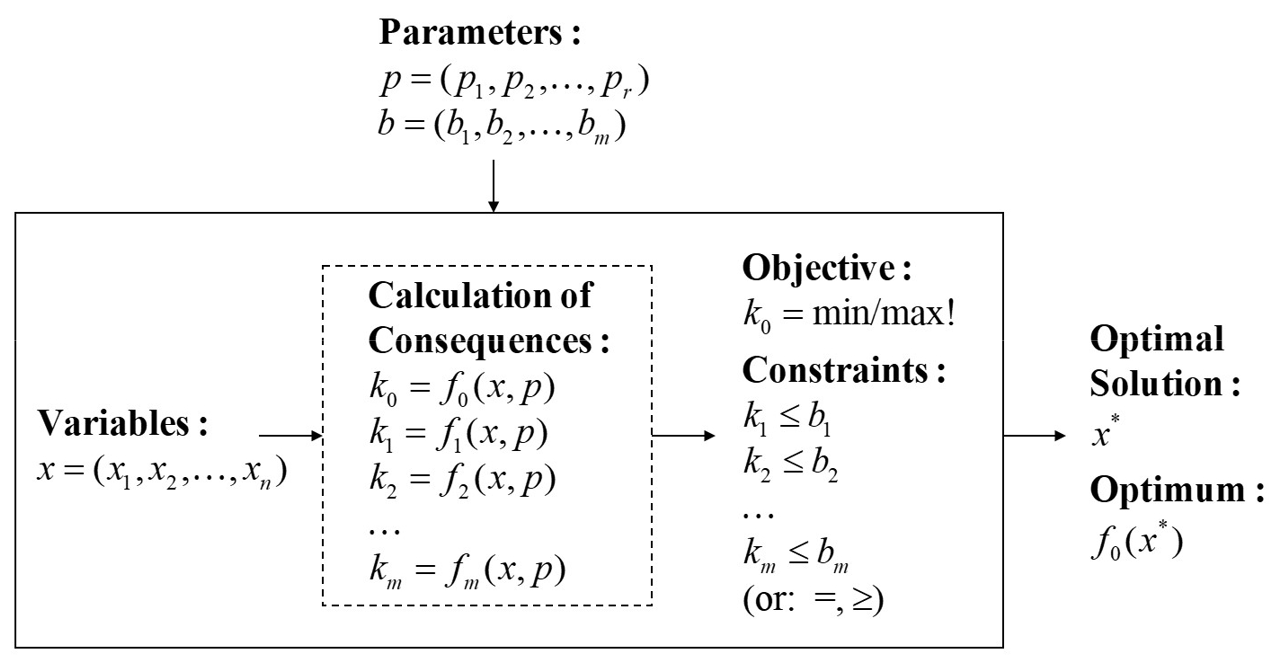
\includegraphics[width=0.5\textwidth]{figures/optimization_model.png}
\caption{Optimization Model}
\end{figure}

\textit{Model itself does not calculate solution: Optimization algorithms needed}

\subsubsection{Example Optimization Model}

\begin{figure}[H]
\centering
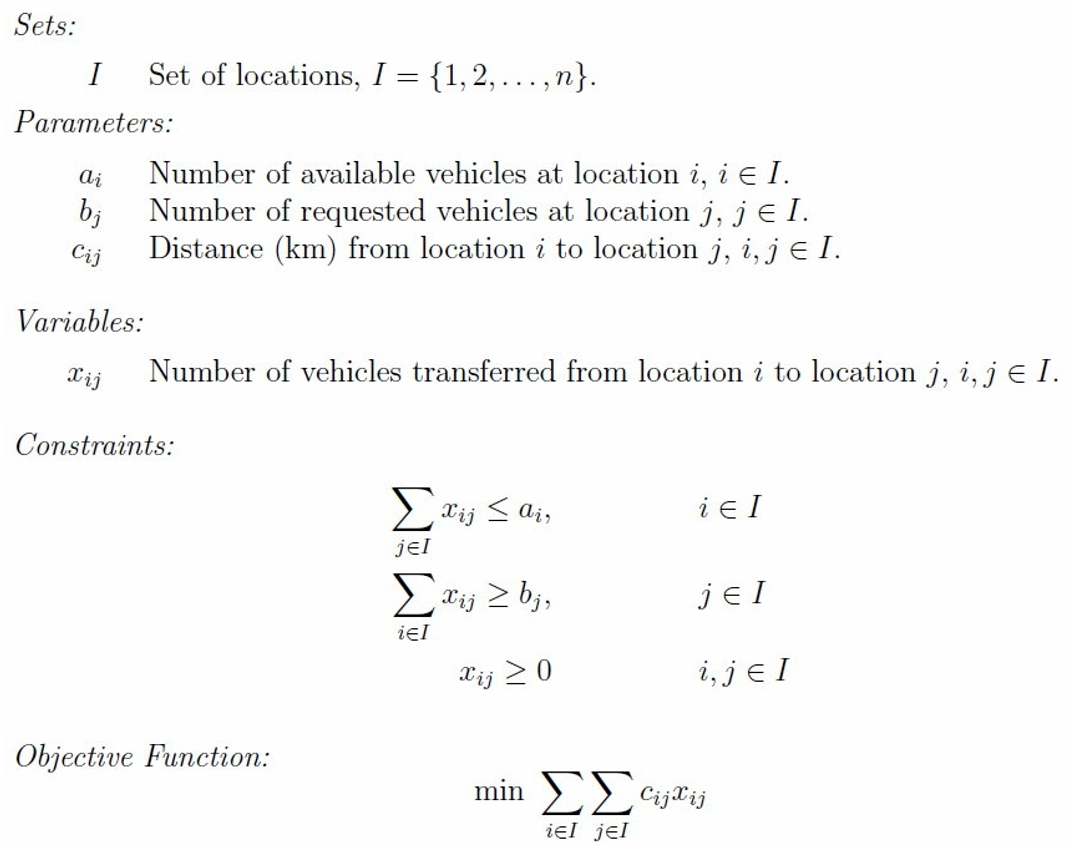
\includegraphics[width=0.6\textwidth]{figures/example_optimization_model.png}
\caption{Example for an optimization model}
\end{figure}

\subsection{Problem Formulation}

\begin{figure}[H]
\centering
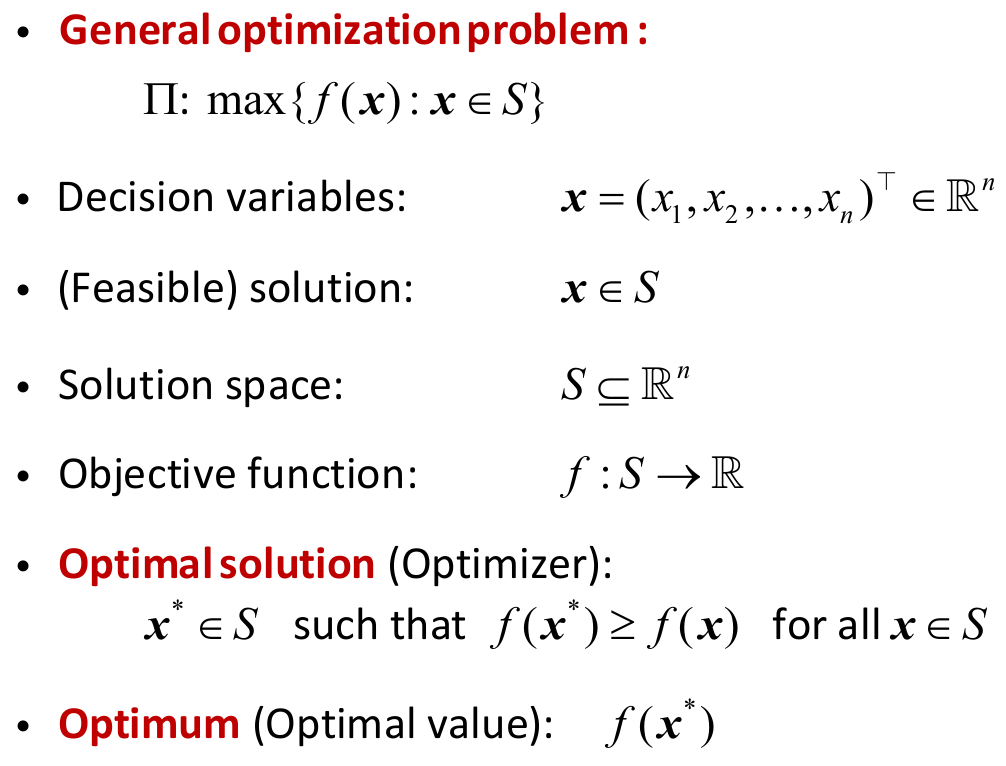
\includegraphics[width=0.5\textwidth]{figures/problem_formulation.png}
\caption{Discrete Optimization - Problem formulation}
\end{figure}

\subsection{Definition of Solution Space}
\textbf{Functional Constraints} \\
e.g. $S = \{x \in R \times Z \times \{0,1\}:x_1 + x_2 + x_3 = 1, x \geq 0\}$ \\
$x = (x_1, x_2, x_3)^T$ and $x_1 \in R$, $x_2 \in Z$, $x_3 \in \{0,1\}$

\textbf{Non-Functional Constraints} \\
e.g. $S = \{x \in Z^n$ : x is a permutation of 1 ... n \} $\Rightarrow$ Hard to solve! \\
The non-functional constraint is just describing the problem.

\subsection{Problems and Problem Instances}
\begin{figure}[H]
\centering
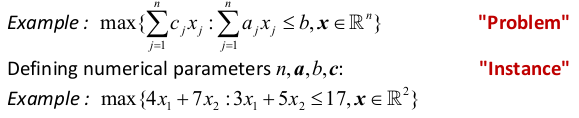
\includegraphics[width=0.5\textwidth]{figures/problemandinstance.png}
\caption{Discrete Optimization - Problem and Problem Instances}
\end{figure}

\subsection{Neighborhoods}
\begin{figure}[H]
\centering
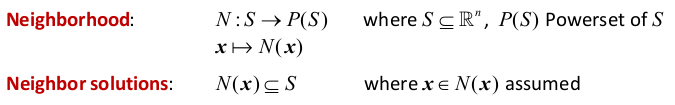
\includegraphics[width=0.5\textwidth]{figures/neighborhood.png}
\caption{Discrete Optimization - Neighborhood}
\end{figure}

A neighborhood is a set of subsets of the powerset, where the subsets are neighbors of x. For instance, if the neighborhood of 1 is 1 and 3, we write $N(1) = \{1, 3\}$.

\begin{tcolorbox}[colback=red!5!white,colframe=red!75!black]
If we have a feasible Solution $x \in S$, we search in the neighborhood for a better solution. If we don't find any better solution in this neighborhood, we have a local optimum. \\
Doing so and repeating the search in the neighborhoods is called \textbf{Principle of Local Search Methods or Trajectory - Based Search}.
\end{tcolorbox}

\subsection{Some Topological Notes}
\textbf{Interior Point:} Point within the boundary, NOT on the boundary \\
\textbf{Boundary Point:} Point on the boundary \\
\textbf{Closed:} All boundary points of S are in S \\
\textbf{Open:} All points are interior points

\subsection{Convex Optimization}

The following pictures shows us different possibilities for convex problems.

\begin{figure}[H]
\centering
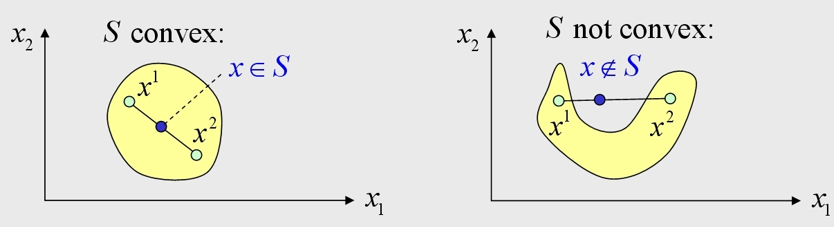
\includegraphics[width=0.5\textwidth]{figures/convexOptimization1.png}
\caption{Discrete Optimization - Convex Optimization Problem 1}
\end{figure}

\begin{figure}[H]
\centering
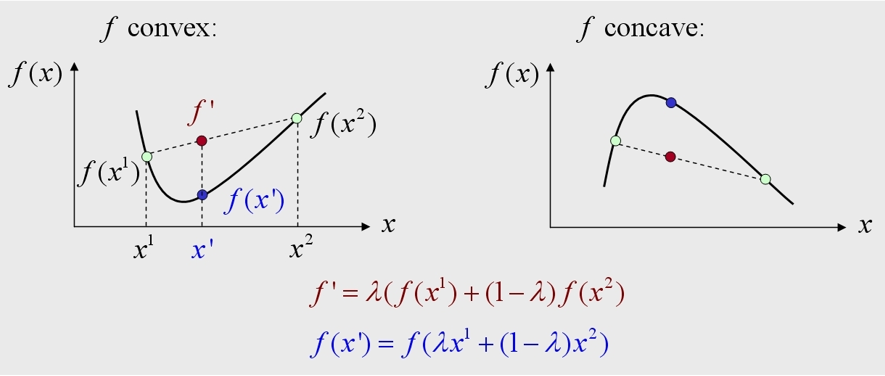
\includegraphics[width=0.5\textwidth]{figures/convexOptimization2.png}
\caption{Discrete Optimization - Convex Optimization Problem 2}
\end{figure}

\begin{figure}[H]
\centering
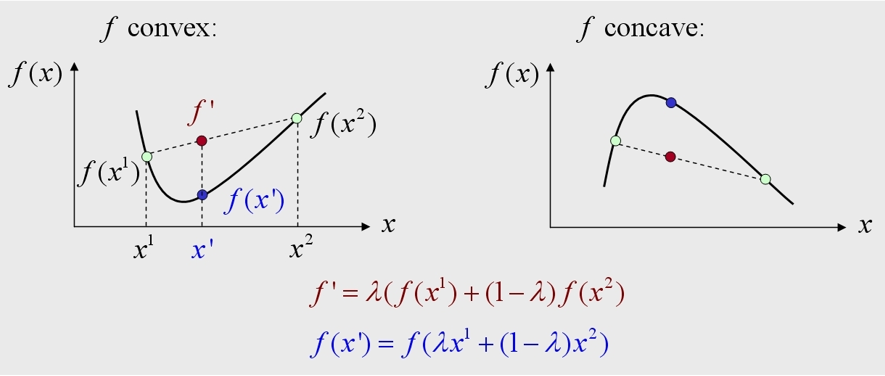
\includegraphics[width=0.5\textwidth]{figures/convexOptimization2.png}
\caption{Discrete Optimization - Convex Optimization Problem 2}
\end{figure}

\textbf{Convex optimization problem:} \textbf{min}$\{f(x): x \in S\}$ with $f$ \textbf{convex} and $S$ convex \\
\textbf{(Also) Convex optimization problem:} \textbf{max}$\{f(x): x \in S\}$ with $f$ \textbf{concave} and $S$ convex

\begin{tcolorbox}[colback=red!5!white,colframe=red!75!black]
\textbf{Theorem}: In convex optimization problem, local optimum is global optimum.\\
\textbf{Theorem}: Consider max$\{f(x) : x \in S\}$ with $f$ convex und $S$ convex, closed, bounded (or min$\{f(x): x \in S \}$ with $f$ concave): Every local optimum is on boundary.
\end{tcolorbox}



\clearpage